\documentclass[border=2pt]{standalone}
\usepackage{pgfplots}

\begin{document}
	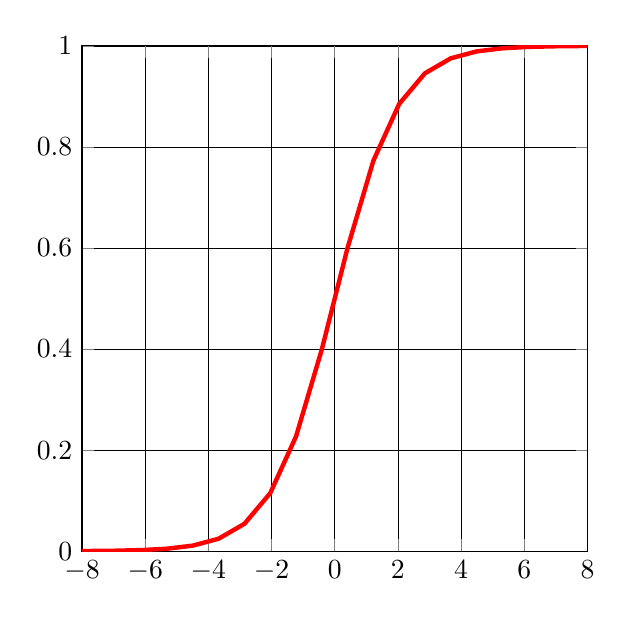
\begin{tikzpicture}[declare function={sigma(\x)=1/(1+exp(-\x));}]
		\begin{axis}[
		xmax=8, 
		xmin=-8, 
		ymin = 0, 
		ymax=1, 
		samples=50, 
		grid=both,
		grid style={line width=.2pt, draw=black},
		width = 8cm,
		height = 8cm,
%		xlabel = Sigmoid Function,
		]	
			
		\addplot[red, ultra thick, domain=-20:20] (x,{sigma(\x)});
		\end{axis}
	\end{tikzpicture}
\end{document}